\section{Discussion}\label{Discussion}
\subsection{How long should auscultate for?}
The optimal input length for heart sounds in AI models is a subject of debate. Cardiac auscultation offers significant predictive value for cardiac diagnosis, characterized by its rapid and cost-effective nature \cite{taylor2015learning}. In the PhysioNet 2016 dataset, which includes 665 abnormal heart sounds and 2575 normal heart sounds, the lengths of recordings range from 3 seconds to 60 seconds. Meanwhile, the Yaseen dataset consists of 1000 abnormal heart sounds and 200 normal heart sounds, all standardized at a length of 2 seconds.

As illustrated in Fig.\ref{FIG:length}, the choice of input length for heart sounds directly impacts the number of cardiac events included, such as S1, diastole, S2, and systole. Fig.\ref{FIG:length.a} demonstrates that a 1.5-second input can theoretically encompass two diastolic and two systolic events. Fig.\ref{FIG:length.b} shows that a 2-second input can include at least two complete cardiac cycles. Fig.\ref{FIG:length.c} reveals that a 3-second input can accommodate three or four full cardiac cycles. 

For the purposes of this paper, the input length is standardized at 3 seconds.
\begin{figure}[!h]
\centering
    % 插入第一张子图
    \begin{subfigure}{.9\linewidth}
        \centering
        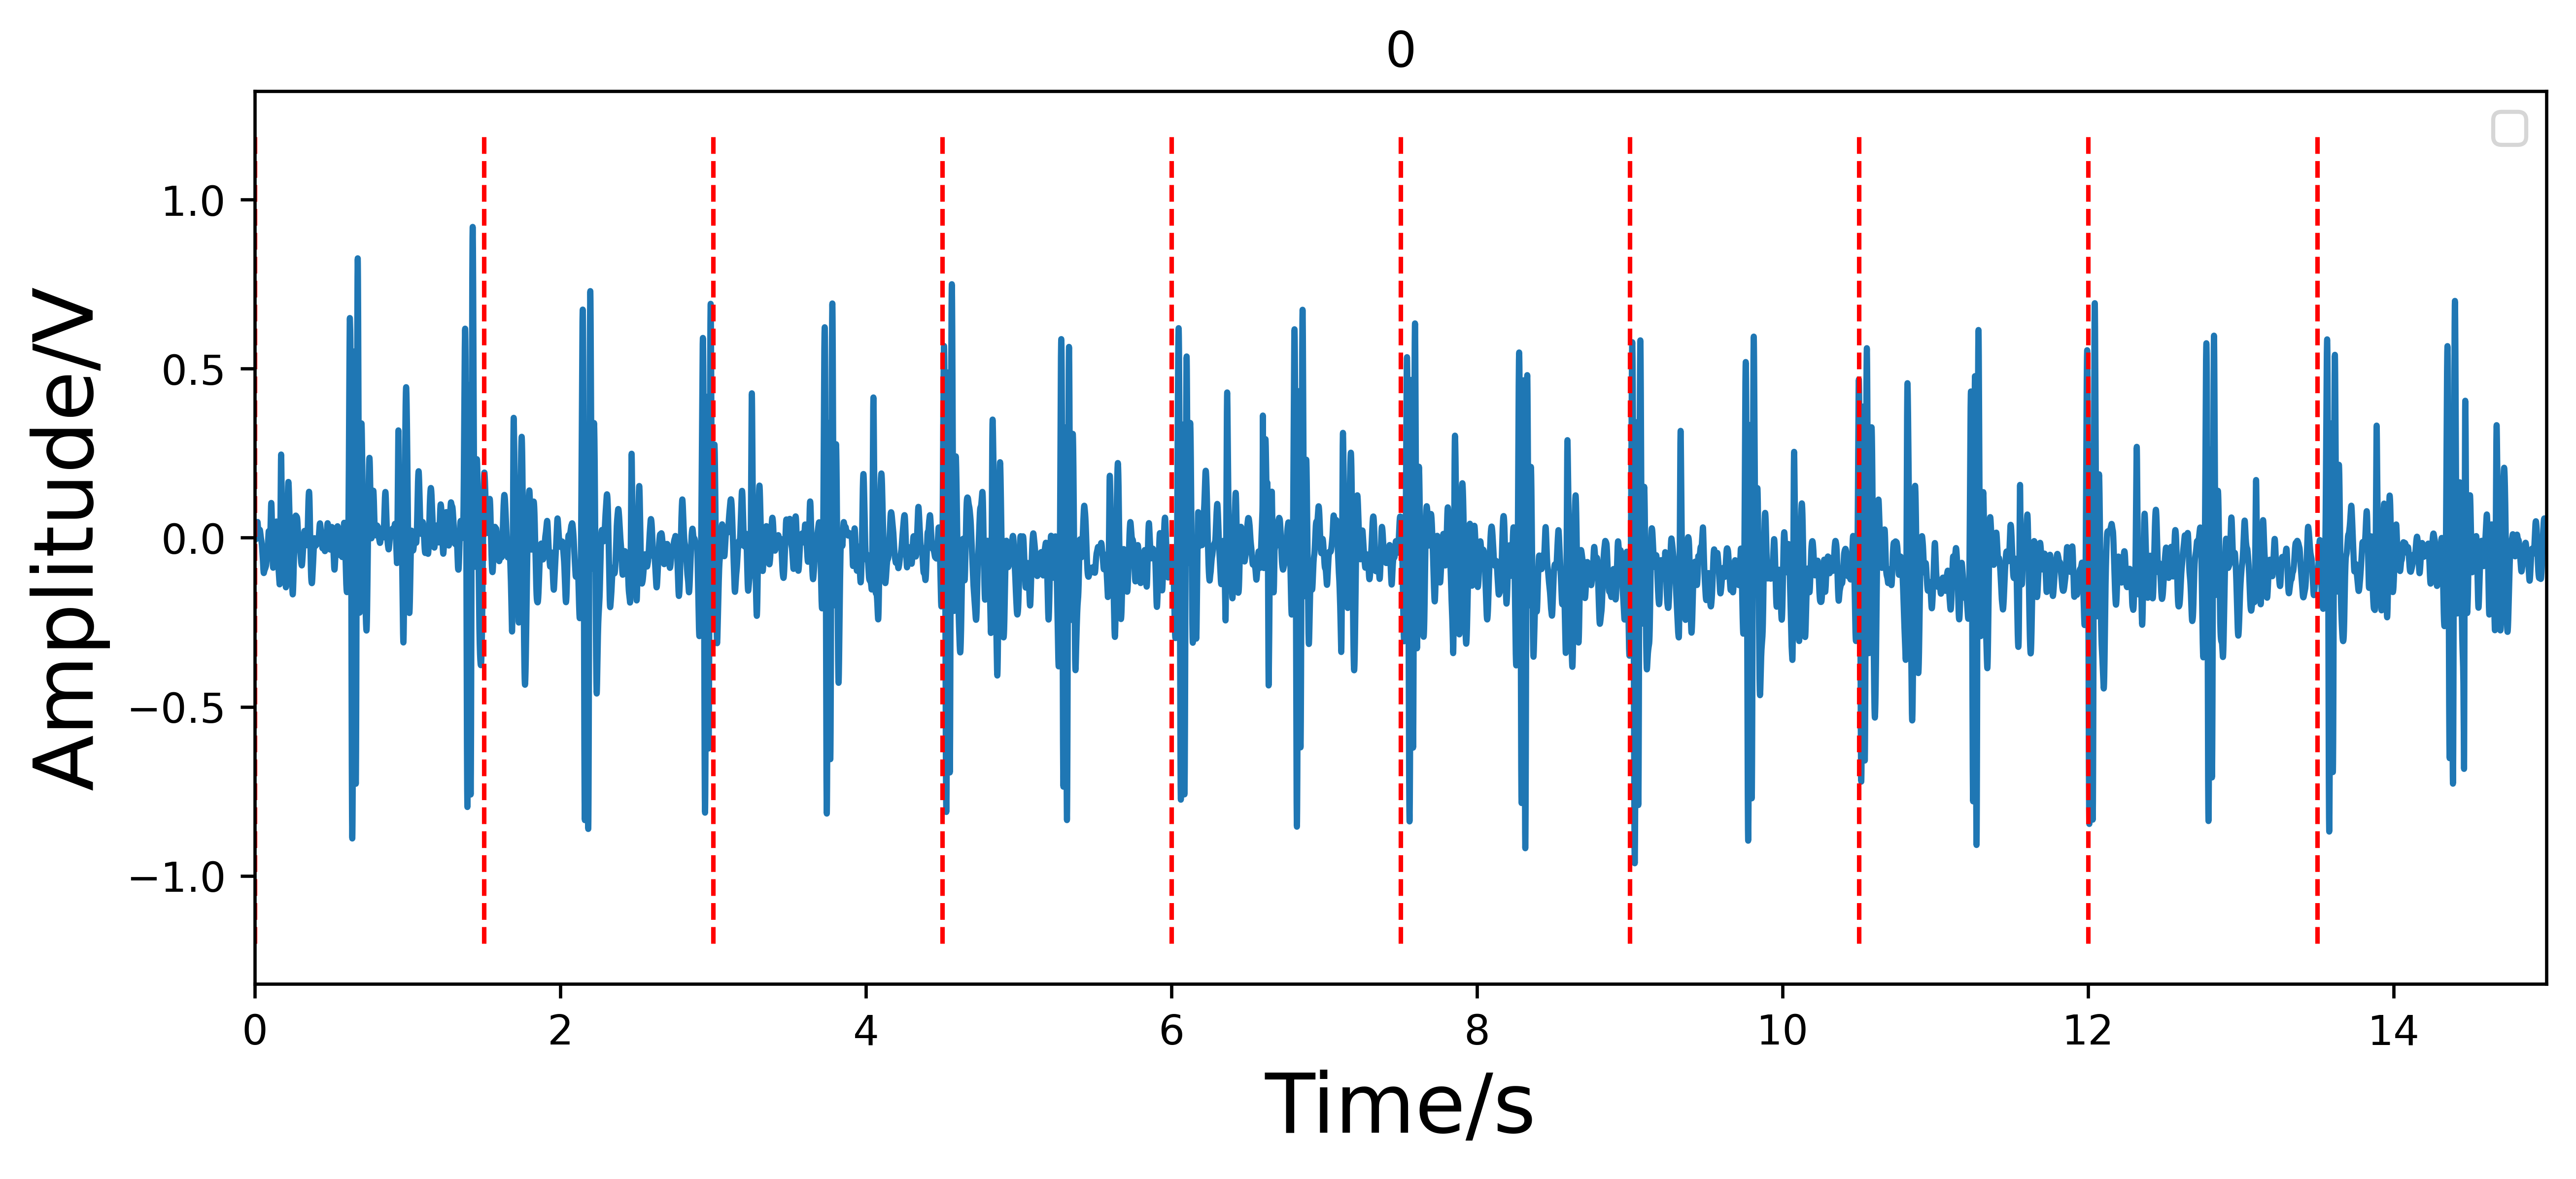
\includegraphics[width=1\linewidth]{figs/disscussion/1.5s.png}
        \caption{Cut with a length of 1.5s}
        \label{FIG:length.a}
    \end{subfigure}\vfill
    % 插入第二张子图
    \begin{subfigure}{.9\linewidth}
        \centering
        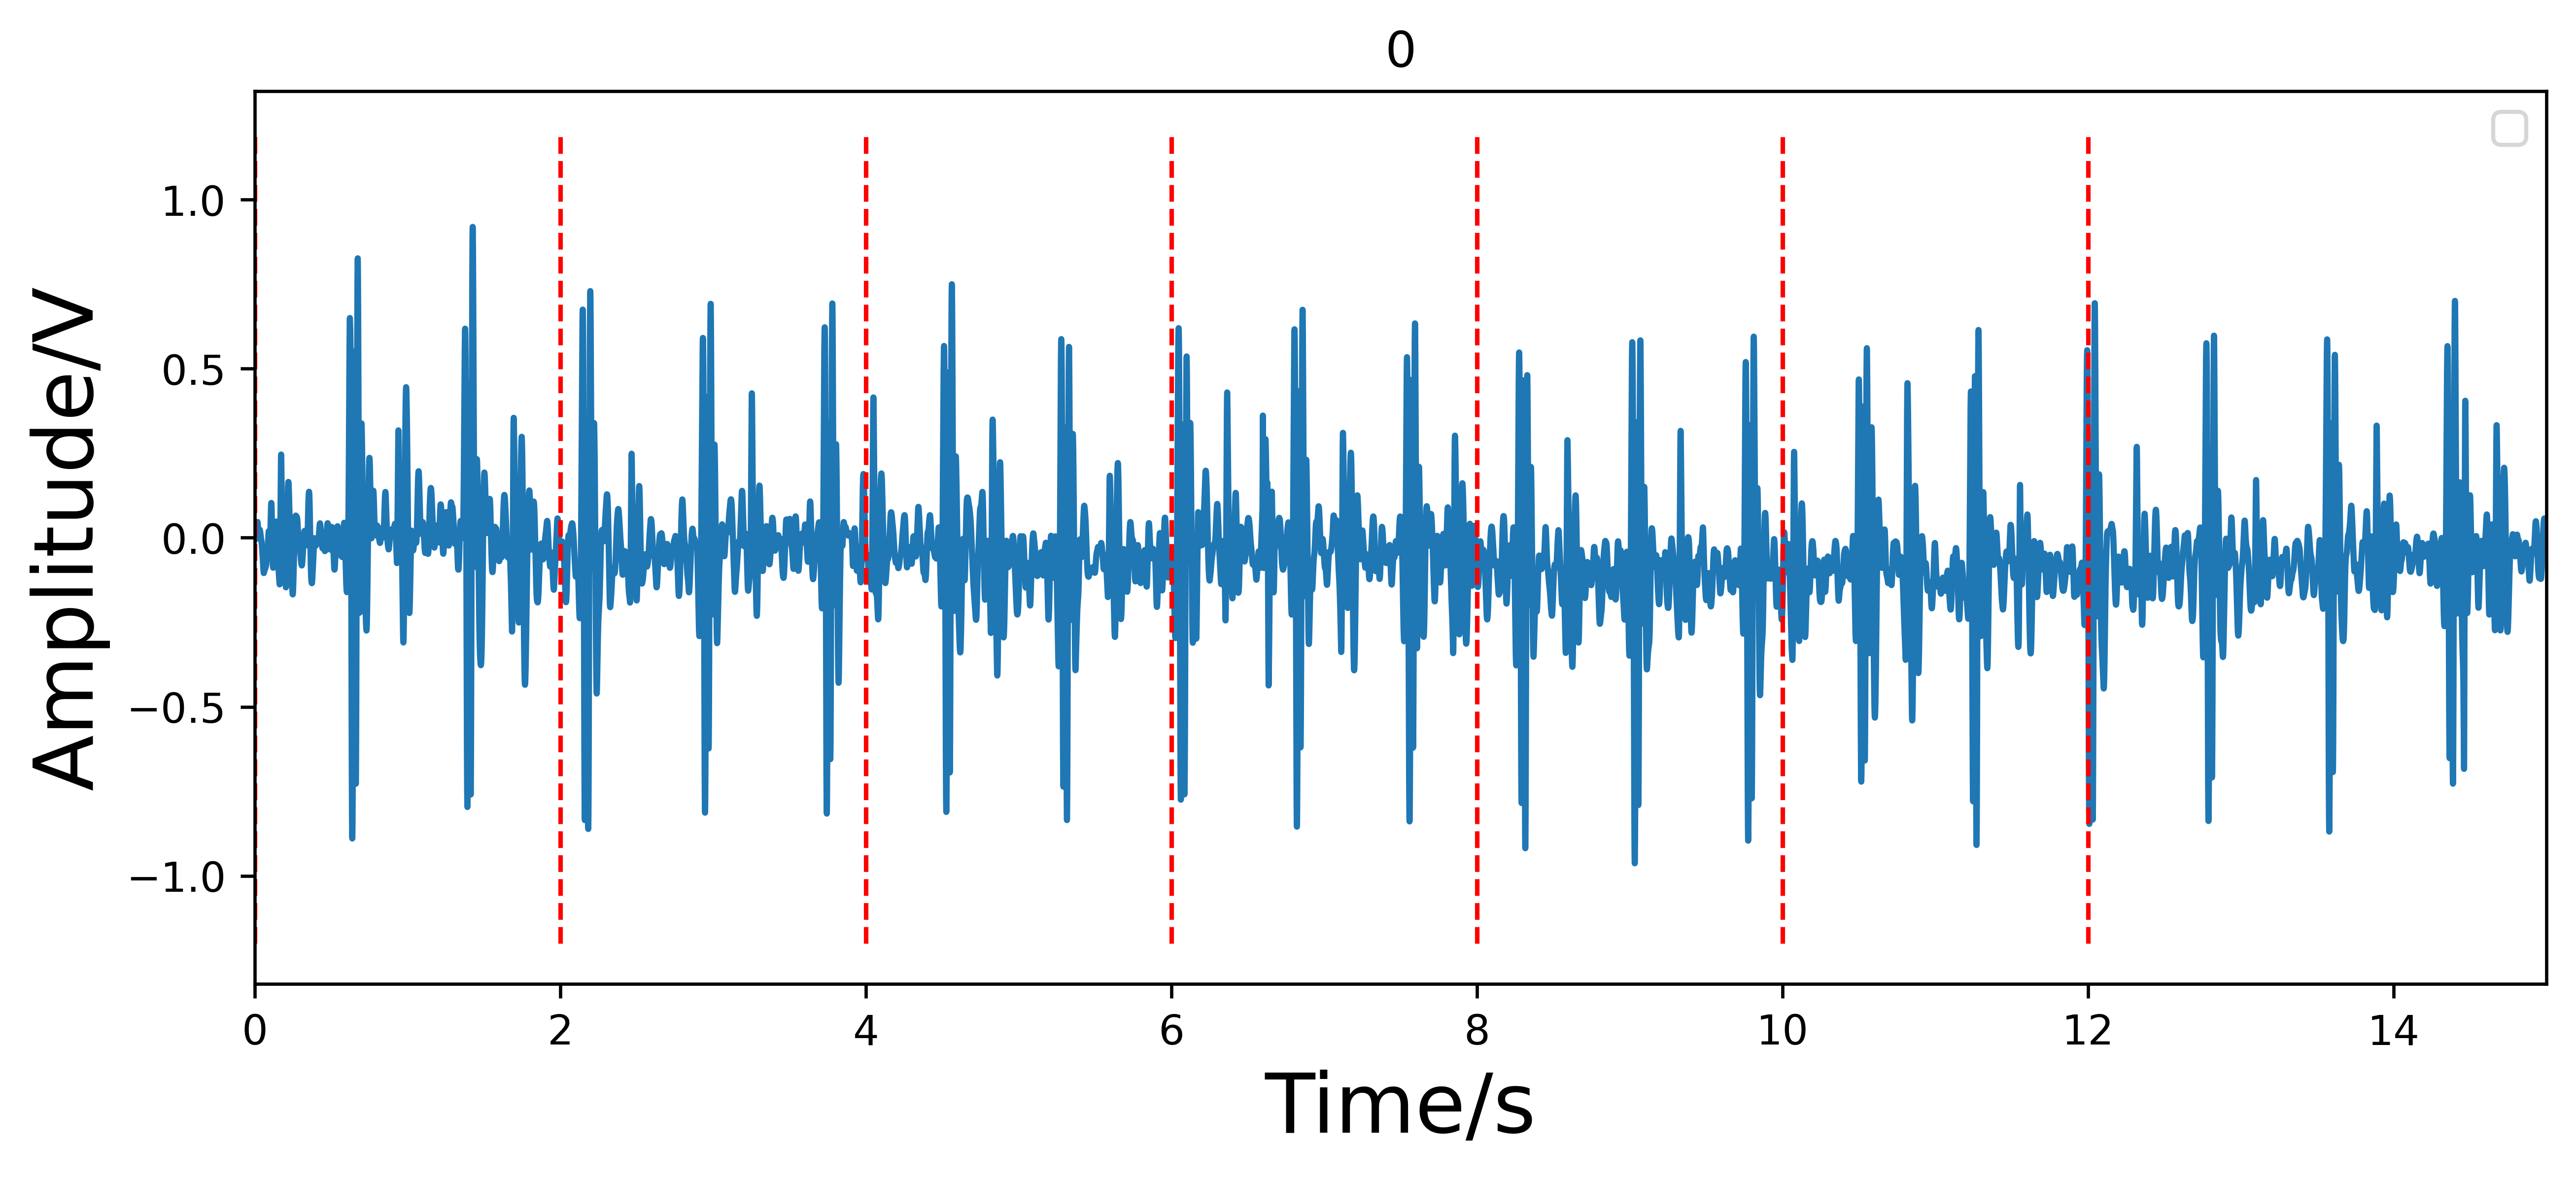
\includegraphics[width=1\linewidth]{figs/disscussion/2s.png}
        \caption{Cut with a length of 2s}
        \label{FIG:length.b}
    \end{subfigure}\vfill
    \begin{subfigure}{.9\linewidth}
        \centering
        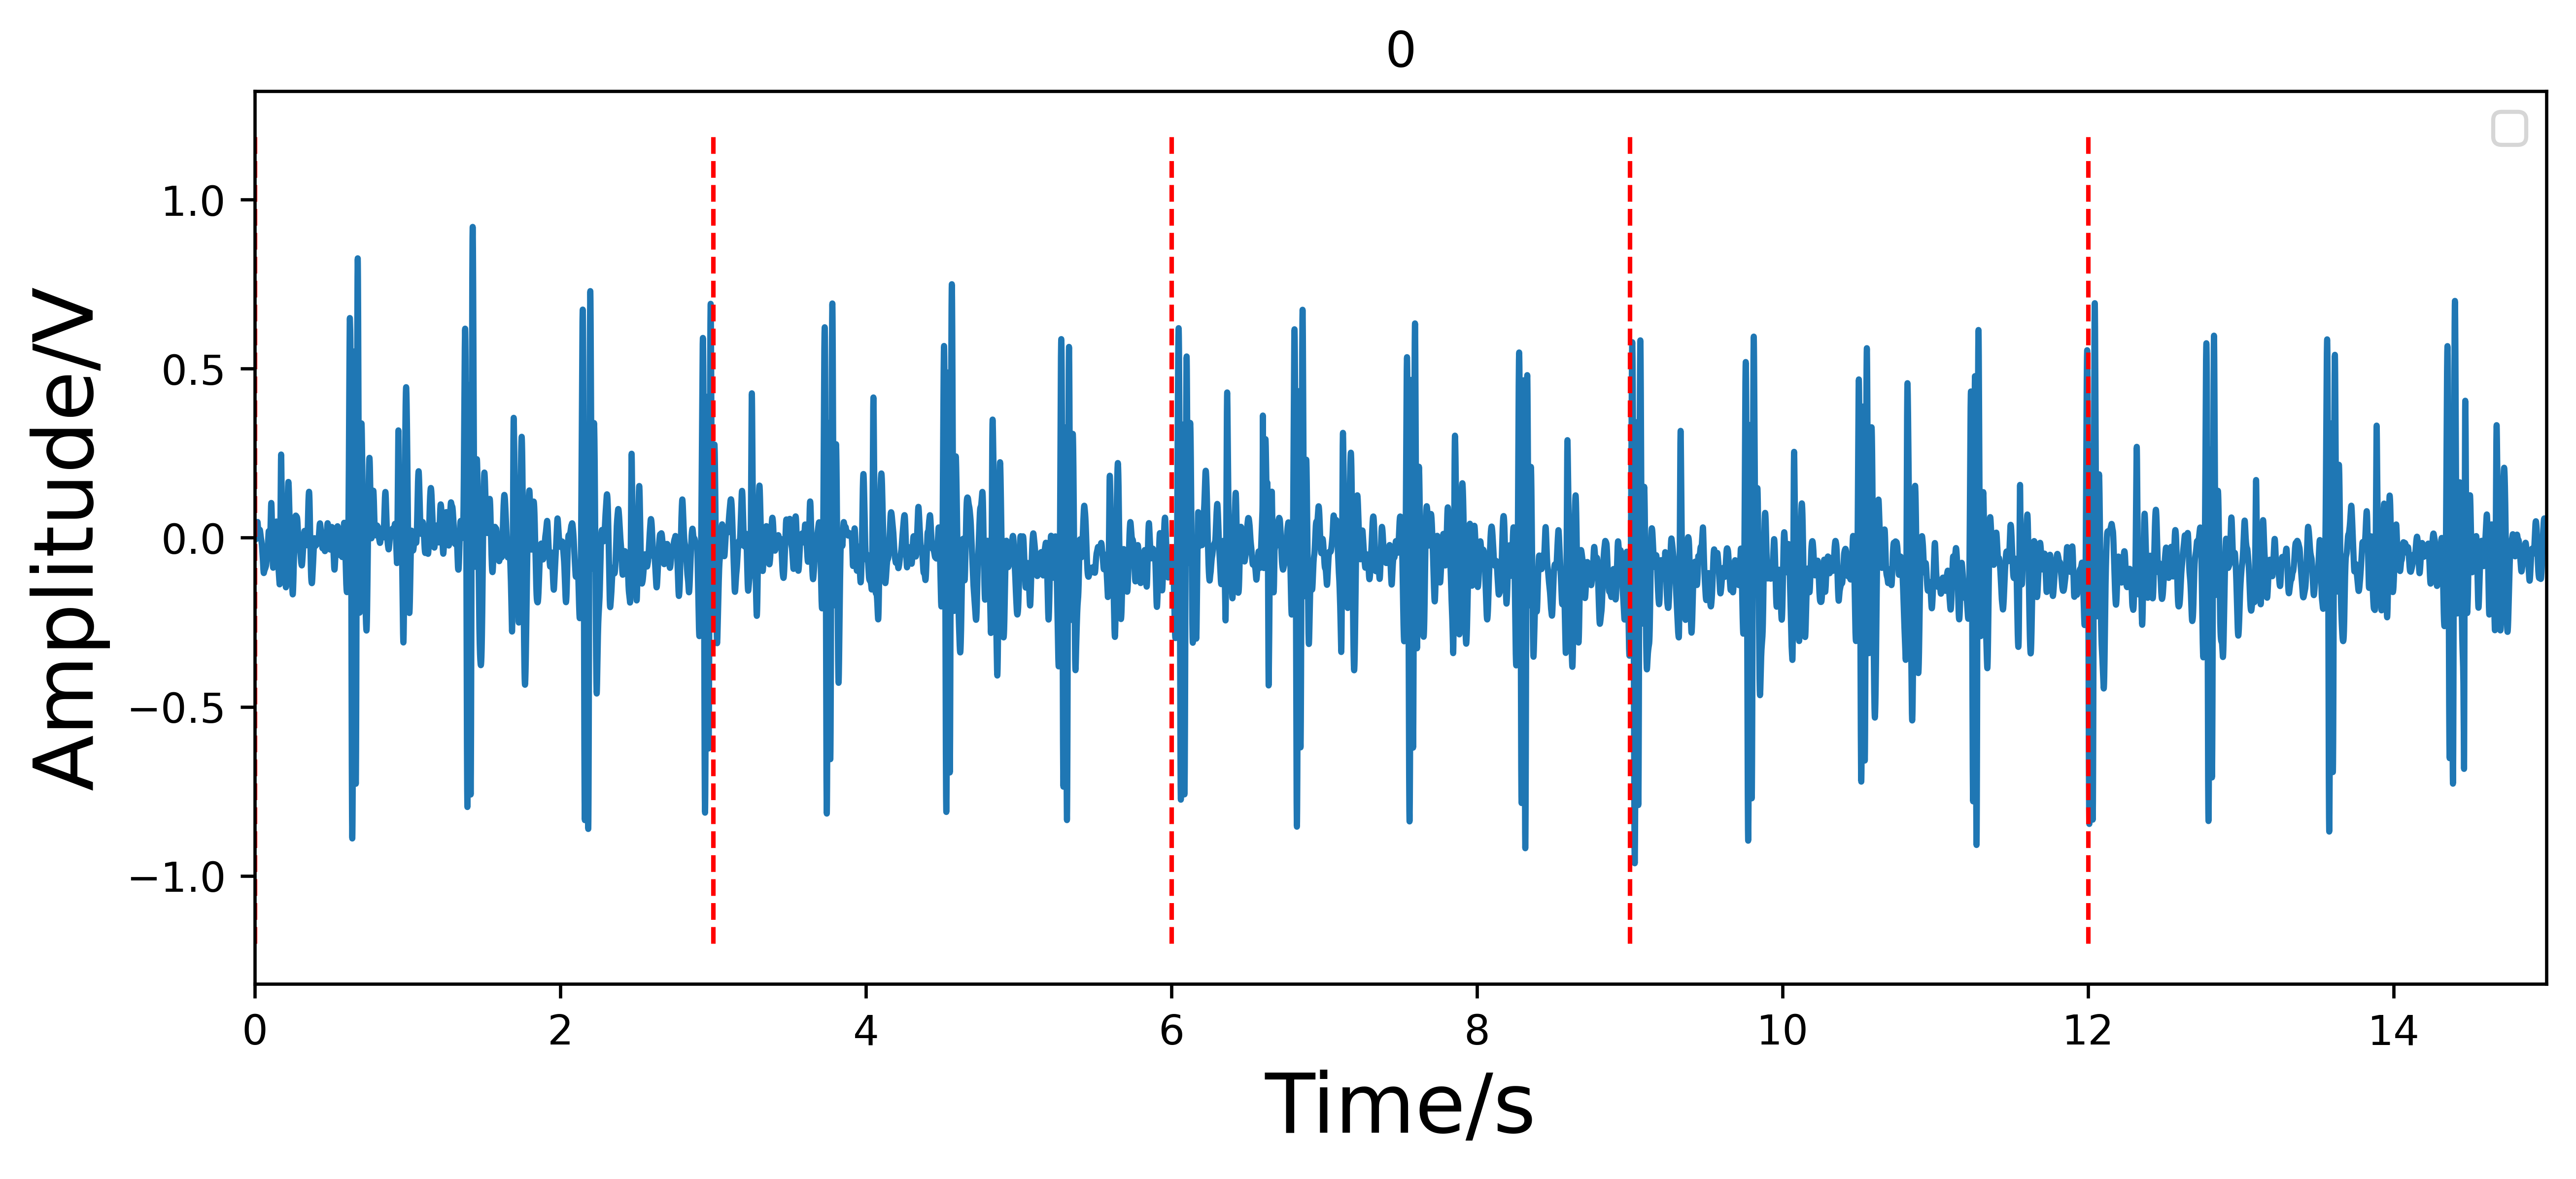
\includegraphics[width=1\linewidth]{figs/disscussion/3s.png}
        \caption{Cut with a length of 3s}
        \label{FIG:length.c}
    \end{subfigure}
\caption{\textbf{Effect of different cutting lengths.} (\textbf{a}) A heart sound is cut with lengths of 1.5s. (\textbf{b}) The same heart sound is cut with lengths of 2s. (\textbf{c}) The same heart sound is cut with lengths of 3s.}
\label{FIG:length}
\end{figure}

\subsection{Interpretability discussion}
Heart sounds contain essential physiological information that reflects the heart's ability to pump blood effectively, and this information is crucial for interpretability in diagnosis. In this study, we analyze the time-frequency characteristics of heart sounds using short-term Fourier transforms (STFT), with a primary focus on the mitral valve, located at the point of the strongest apical beat, to provide a more intuitive explanation.

As illustrated in Fig.\ref{FIG:Time&Frequency.a}, the stable S1 amplitude is predominantly concentrated within the 100 Hz frequency range, clearly reflecting the normal function of the mitral valve. In contrast, the aortic valve, located in the second intercostal space at the right sternal border, is situated further from the heart and is influenced by lung sounds, resulting in a lower signal amplitude. This variation can be explained by the attenuation of energy during sound propagation. The pulmonic valve, positioned in the second intercostal space at the left sternal border, exhibits signal characteristics that are intermediate between those of the mitral and aortic valves, further illustrating the impact of different heart valve locations on heart sound characteristics.

Heart sounds from the mitral valve were collected from the same patient both before and after receiving initial medical intervention, as shown in Fig.\ref{FIG:Time&Frequency.d} and Fig.\ref{FIG:Time&Frequency.e}, providing interpretability of treatment effects. Before treatment, the S1 amplitudes were unstable and were accompanied by noisy lung sounds, indicating impaired heart function. However, after initial treatment, which took place two days later, a noticeable improvement was observed. The heart sound cycle became clearer, and the energy amplitude of S1 was more pronounced, clearly reflecting the positive impact of the treatment on heart function.

\begin{figure*}[h]
\centering
    % 插入第一张子图
    \begin{subfigure}{.3\linewidth}
        \centering
        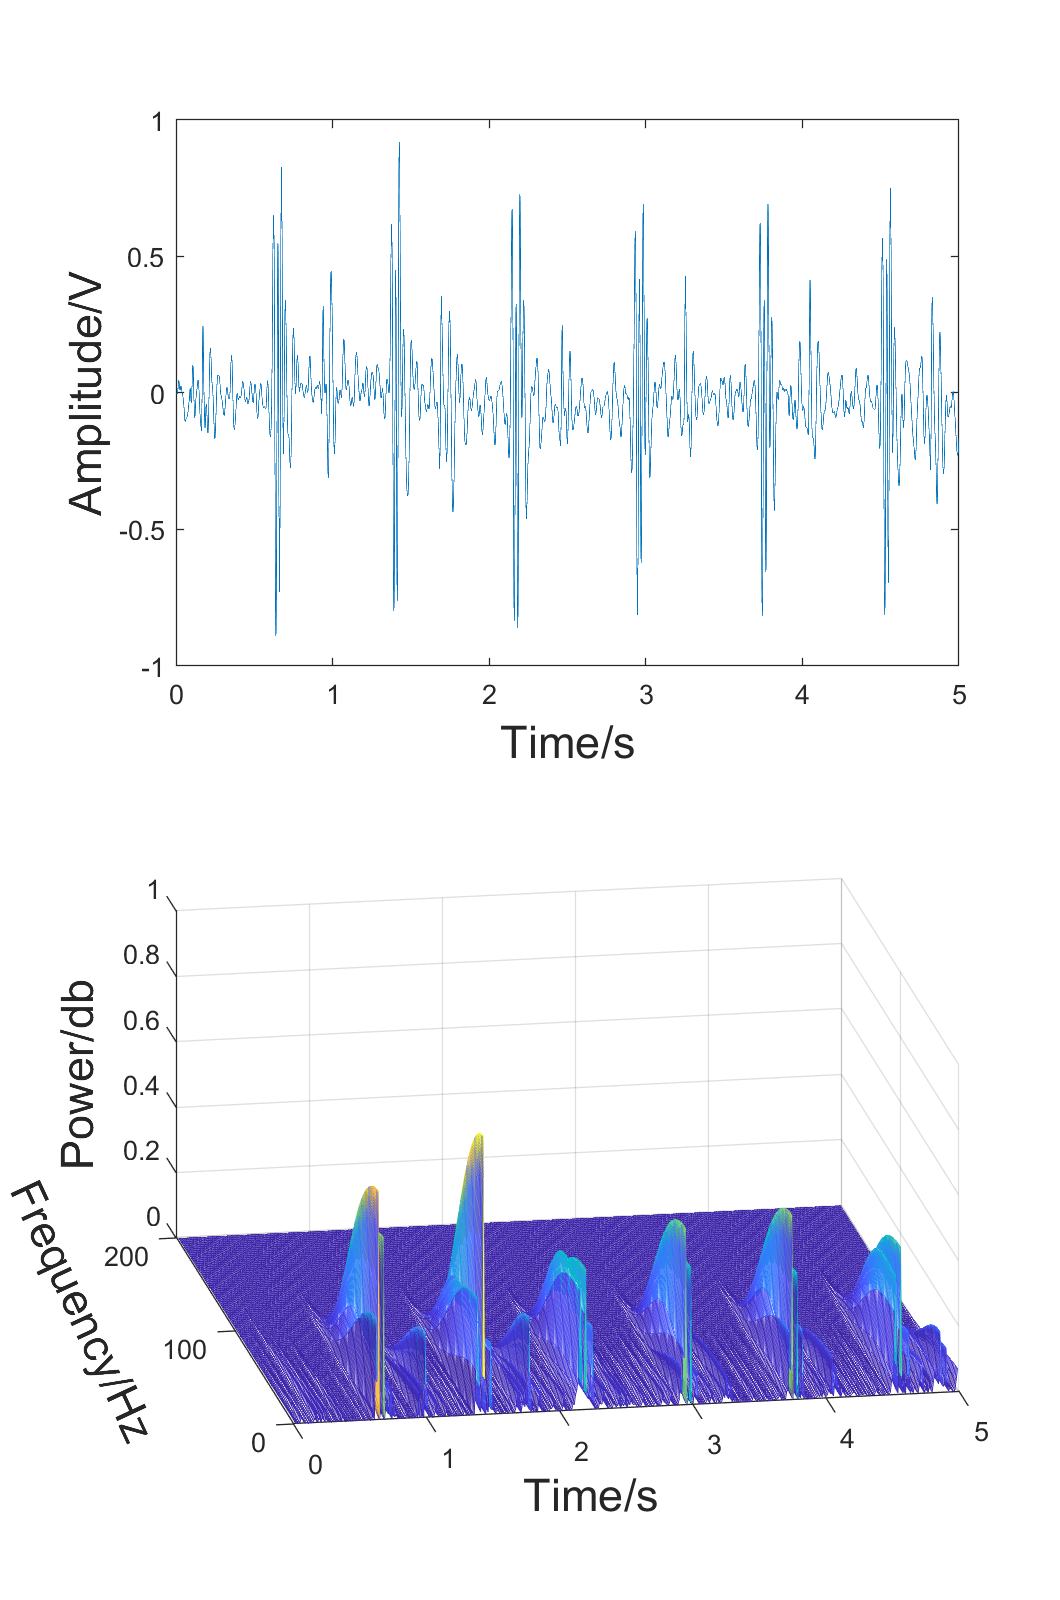
\includegraphics[width=1\linewidth]{figs/disscussion/a.png}
        \caption{Mitral valve}
        \label{FIG:Time&Frequency.a}
    \end{subfigure}\hfill
    % 插入第二张子图
    \begin{subfigure}{.3\linewidth}
        \centering
        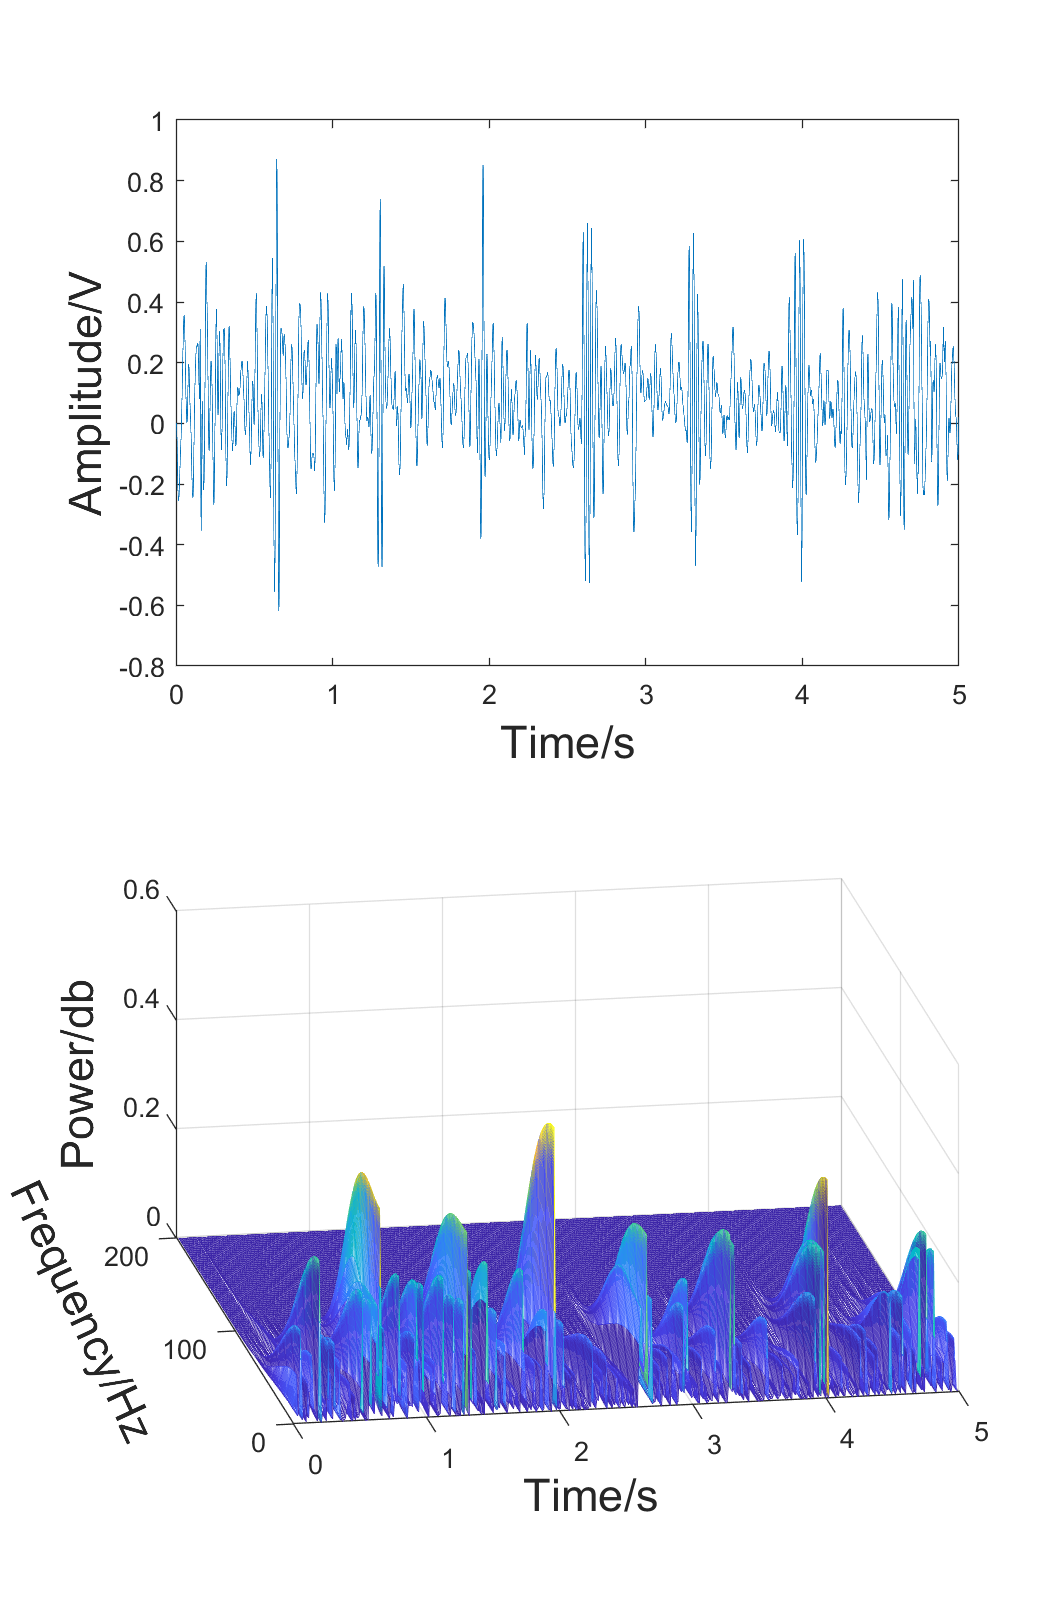
\includegraphics[width=1\linewidth]{figs/disscussion/b.png}
        \caption{Aortic valve}
        \label{FIG:Time&Frequency.b}
    \end{subfigure}\hfill
    \begin{subfigure}{.3\linewidth}
        \centering
        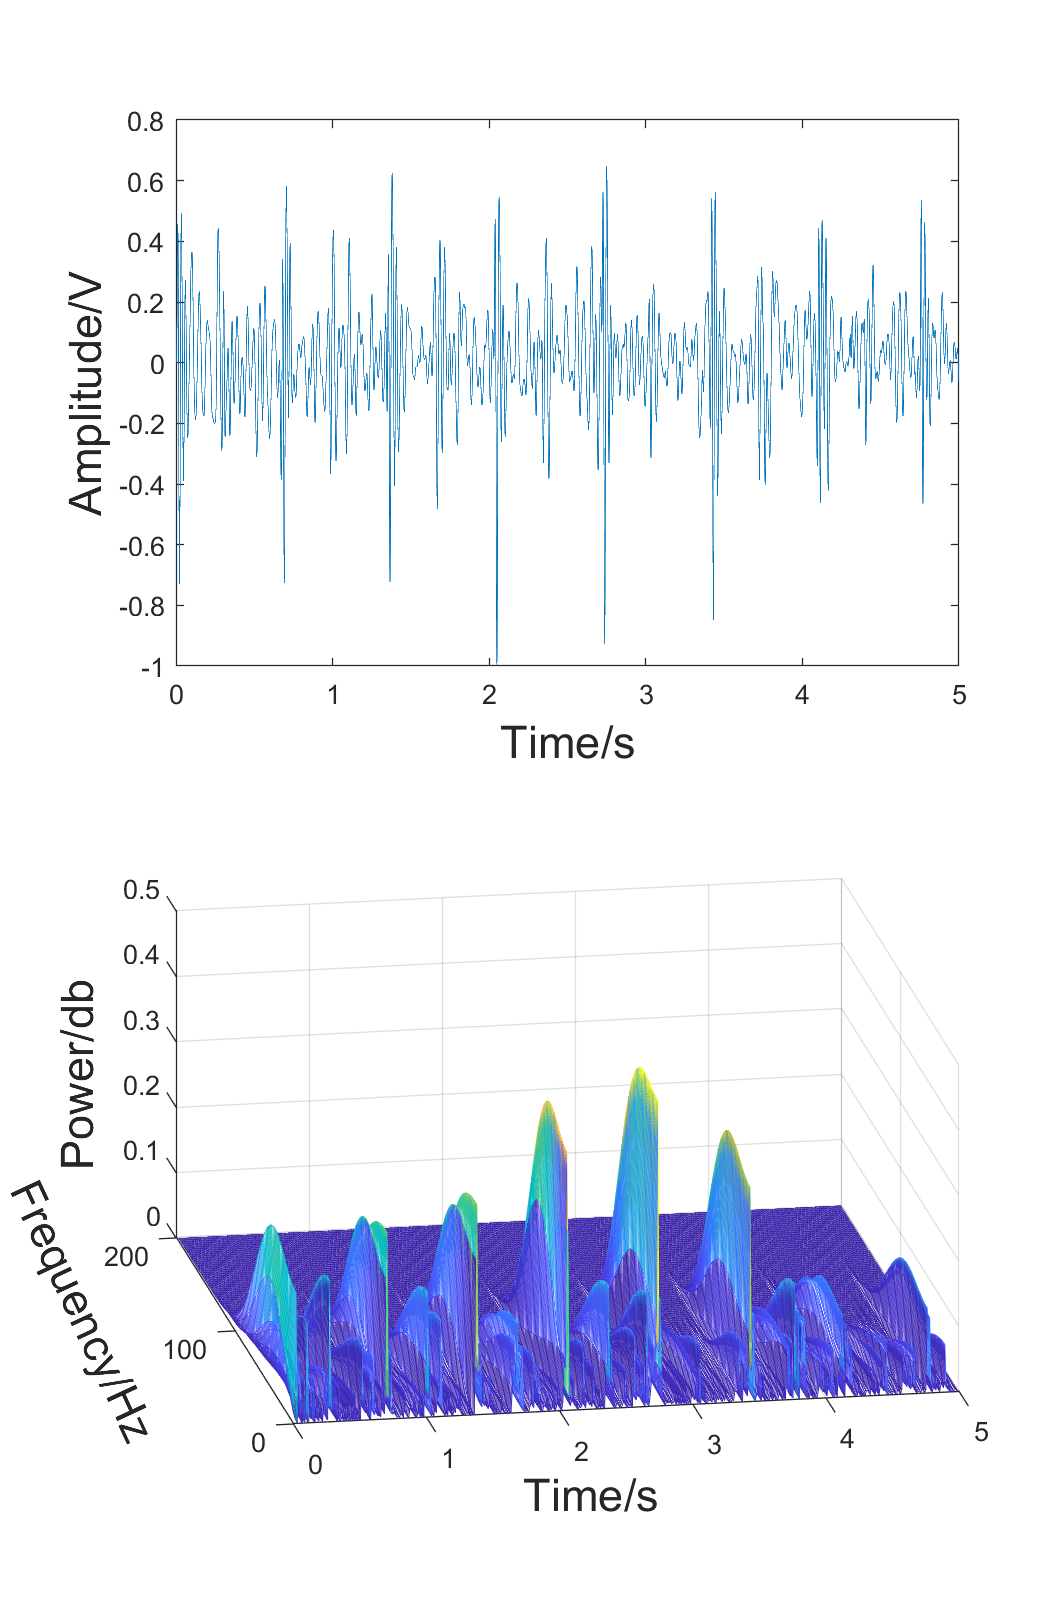
\includegraphics[width=1\linewidth]{figs/disscussion/c.png}
        \caption{Pulmonic valve}
        \label{FIG:Time&Frequency.c}
    \end{subfigure}\\
    \begin{subfigure}{.4\linewidth}
        \centering
        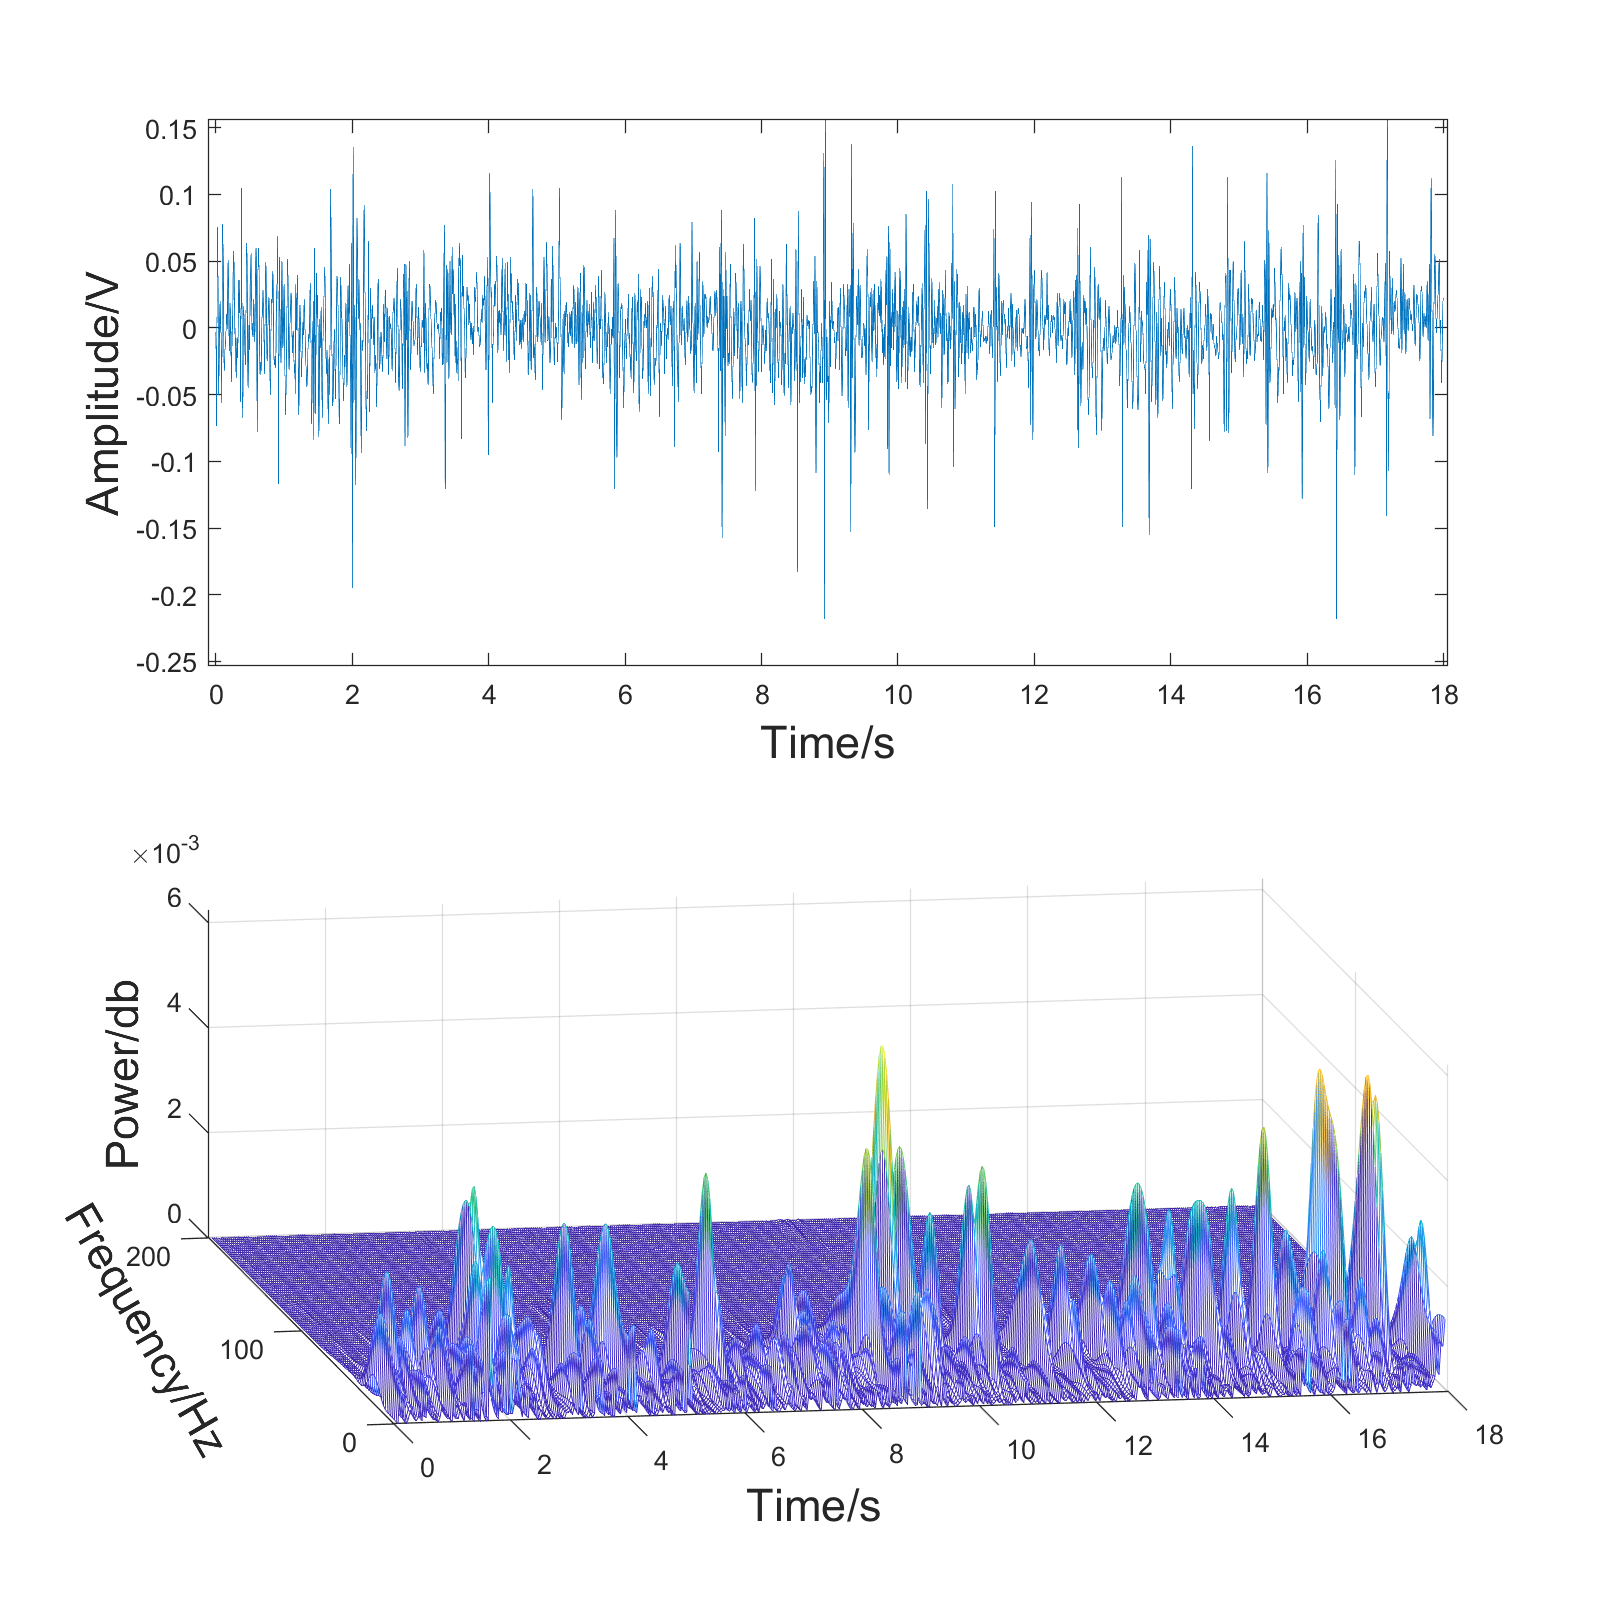
\includegraphics[width=1\linewidth]{figs/disscussion/d.png}
        \caption{Before first-aid}
        \label{FIG:Time&Frequency.d}
    \end{subfigure}\hfill
    % 插入第二张子图
    \begin{subfigure}{.4\linewidth}
        \centering
        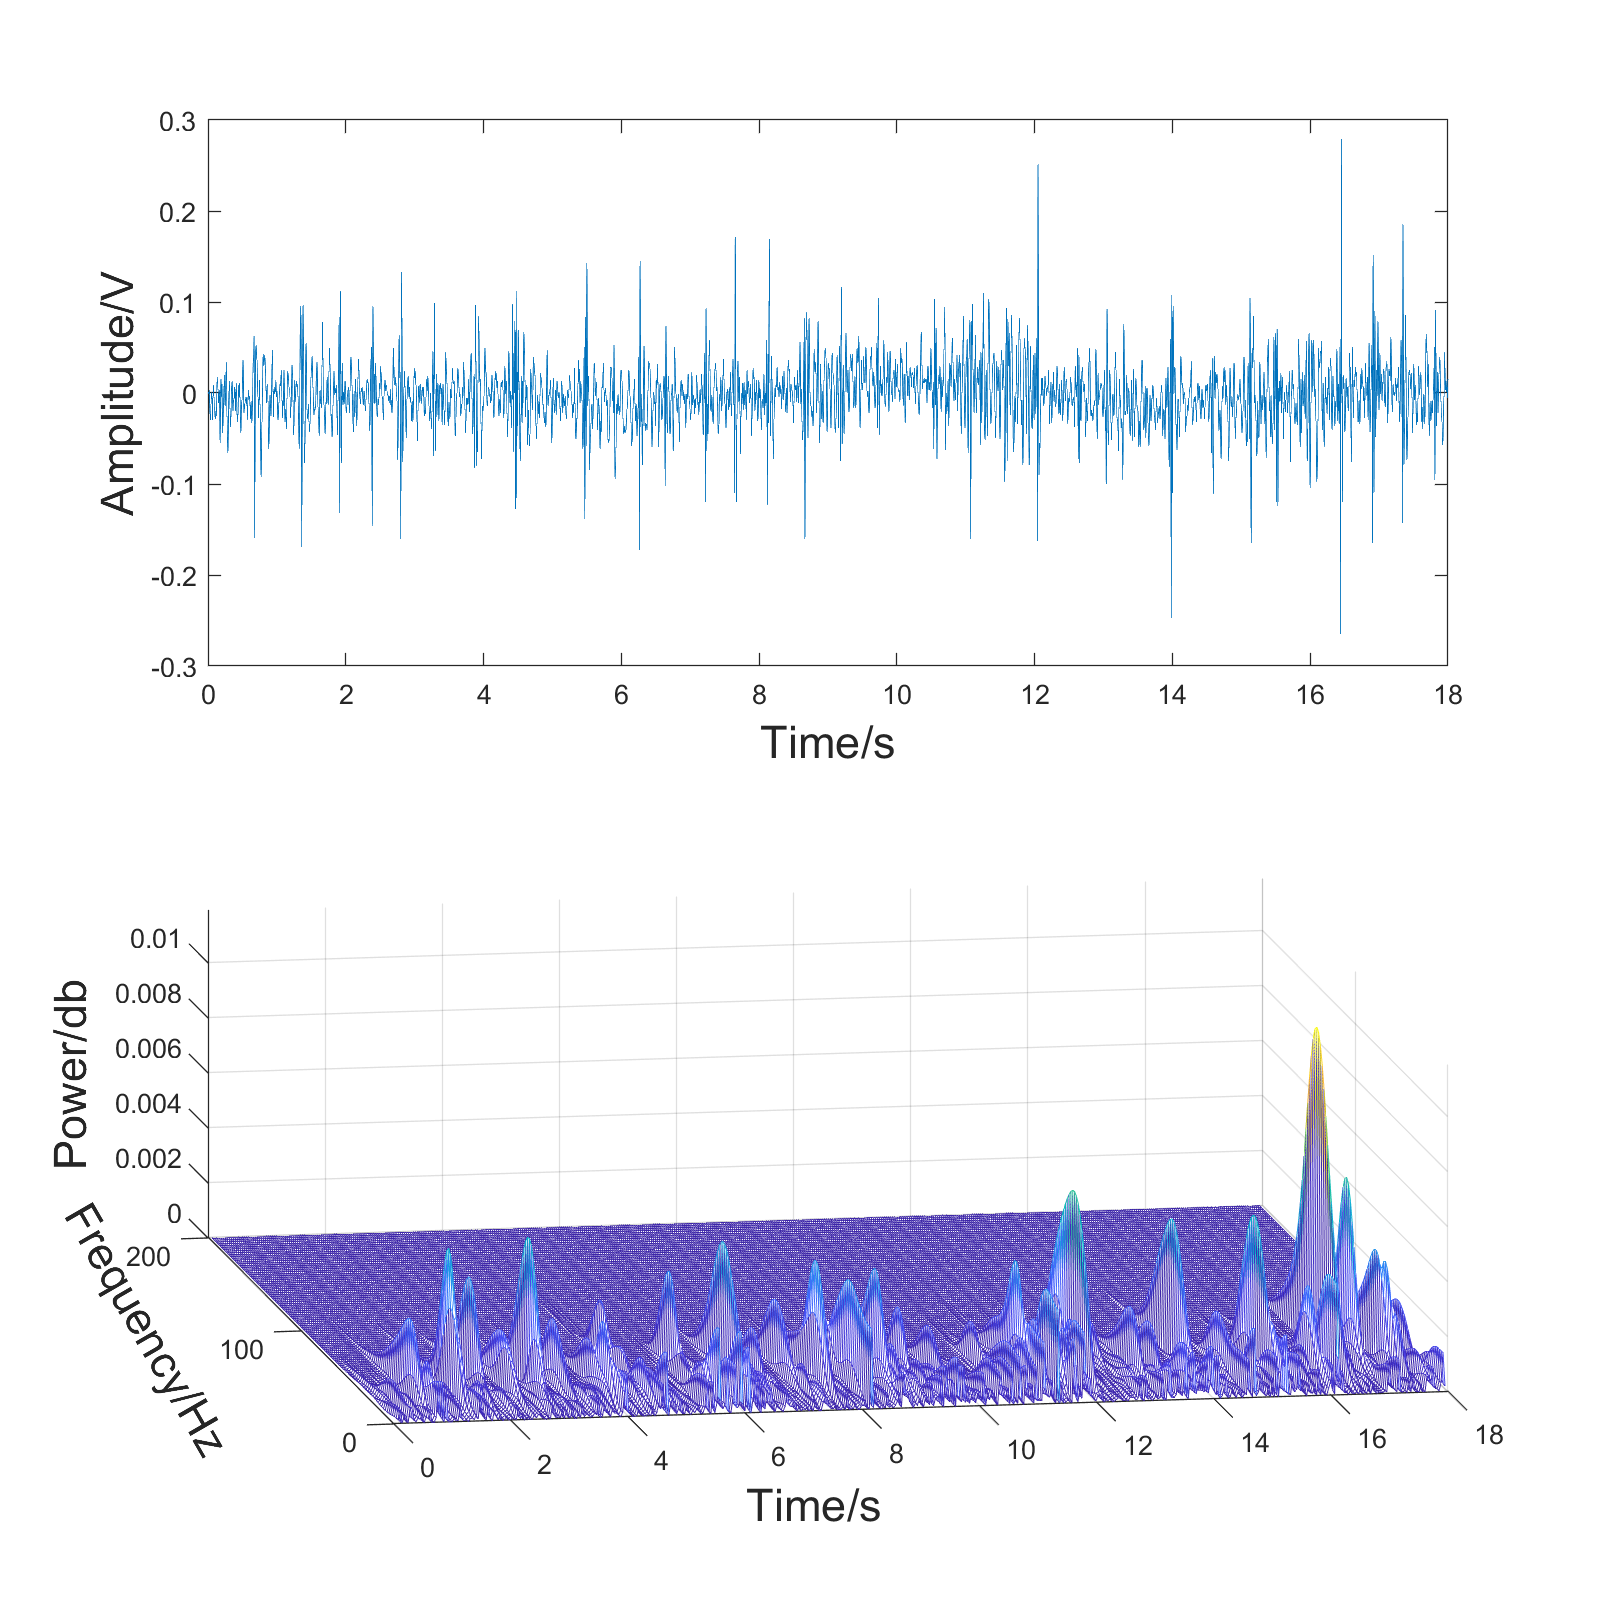
\includegraphics[width=1\linewidth]{figs/disscussion/e.png}
        \caption{After first-aid}
        \label{FIG:Time&Frequency.e}
    \end{subfigure}
\caption{\textbf{Heart sounds in five different situations.} (\textbf{a}) Heart sounds from the mitral valve. (\textbf{b}) Heart sounds from the aortic valve. (\textbf{c}) Heart sounds from the pulmonic valve. (\textbf{d}) Heart sounds before first-aid. (\textbf{e}) Heart sounds after first-aid.}
\label{FIG:Time&Frequency}
\end{figure*}

\subsection{Results discussion}
\subsubsection{Preprocessing and feature extraction}
This paper conducts an in-depth investigation into the optimal decomposition layers, wavelet bases, and threshold shrinkage functions for the denoising of short heart sounds. Fig.\ref{FIG:wavelet} presents our findings, indicating that a 7-layer decomposition using the $f_{self}$ threshold based on the sym8 wavelet yields the most effective denoising results. It's worth noting that Db6 and sym8 wavelets exhibit similar properties, but sym8, due to its shorter support length and superior energy concentration, is more morphologically aligned with heart sounds.

In contrast to previous studies by Chen \cite{2006Research} and Zhao \cite{2010Research}, this paper employs Signal-to-Noise Ratio (SNR) as the primary metric for evaluating noise reduction, avoiding the limitations of waveform comparison. Additionally, our denoising experiments encompass 26 pathological heart sounds, enhancing the clinical relevance of our findings. Furthermore, in comparison to Cheng \cite{cheng2014denoising}, we propose a new $f_{self}$ construction method that significantly improves SNR (7.8 dB).

As depicted in Fig.\ref{FIG:mfcc}, this study delves into the intricacies of feature extraction, particularly focusing on Mel-spectrum and MFCC. The MFCC feature extraction method for heart sounds possesses the advantage of preserving not only temporal waveform features but also capturing frequency energy distribution. This approach retains valuable information aligned with the Mel scale, which corresponds to human auditory perception.

Fig.\ref{FIG:mfcc.a} illustrates a representation of normal heart sounds, while Fig.\ref{FIG:mfcc.b} showcases an instance of heart sounds from a patient with Mitral Valve Prolapse. Both Mel spectrum and MFCC representations encompass a comprehensive range of waveform characteristics, effectively capturing the intricacies of high-frequency signal features in the form of heat maps.
\begin{figure}[!h]
\centering
    % 插入第一张子图
    \begin{subfigure}{.48\linewidth}
        \centering
        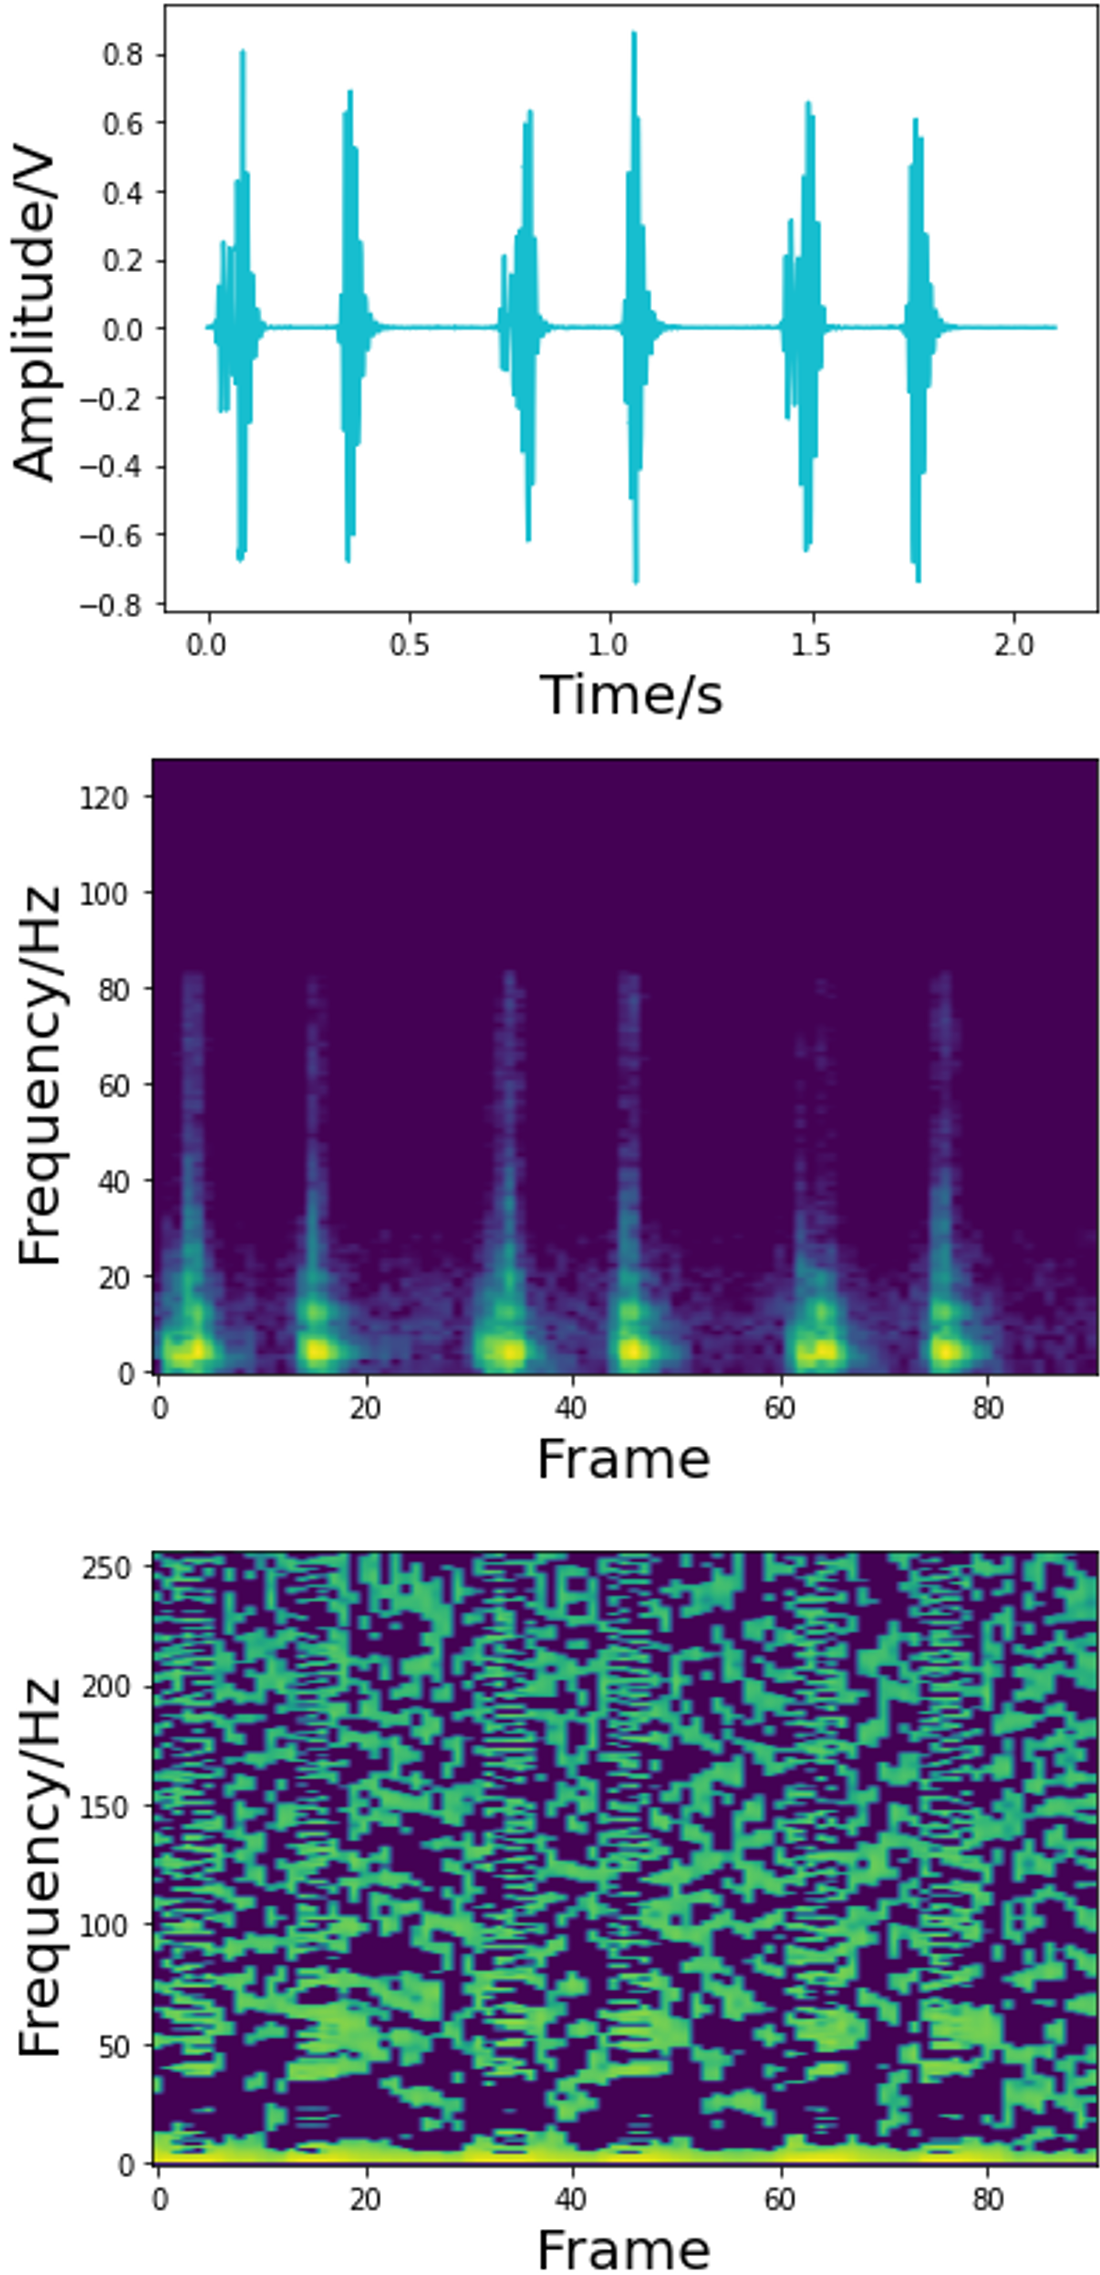
\includegraphics[width=0.99\linewidth]{figs/results/n_mfcc.png}
        \caption{Normal heart sound}
        \label{FIG:mfcc.a}
    \end{subfigure}\hfill
    % 插入第二张子图
    \begin{subfigure}{.48\linewidth}
        \centering
        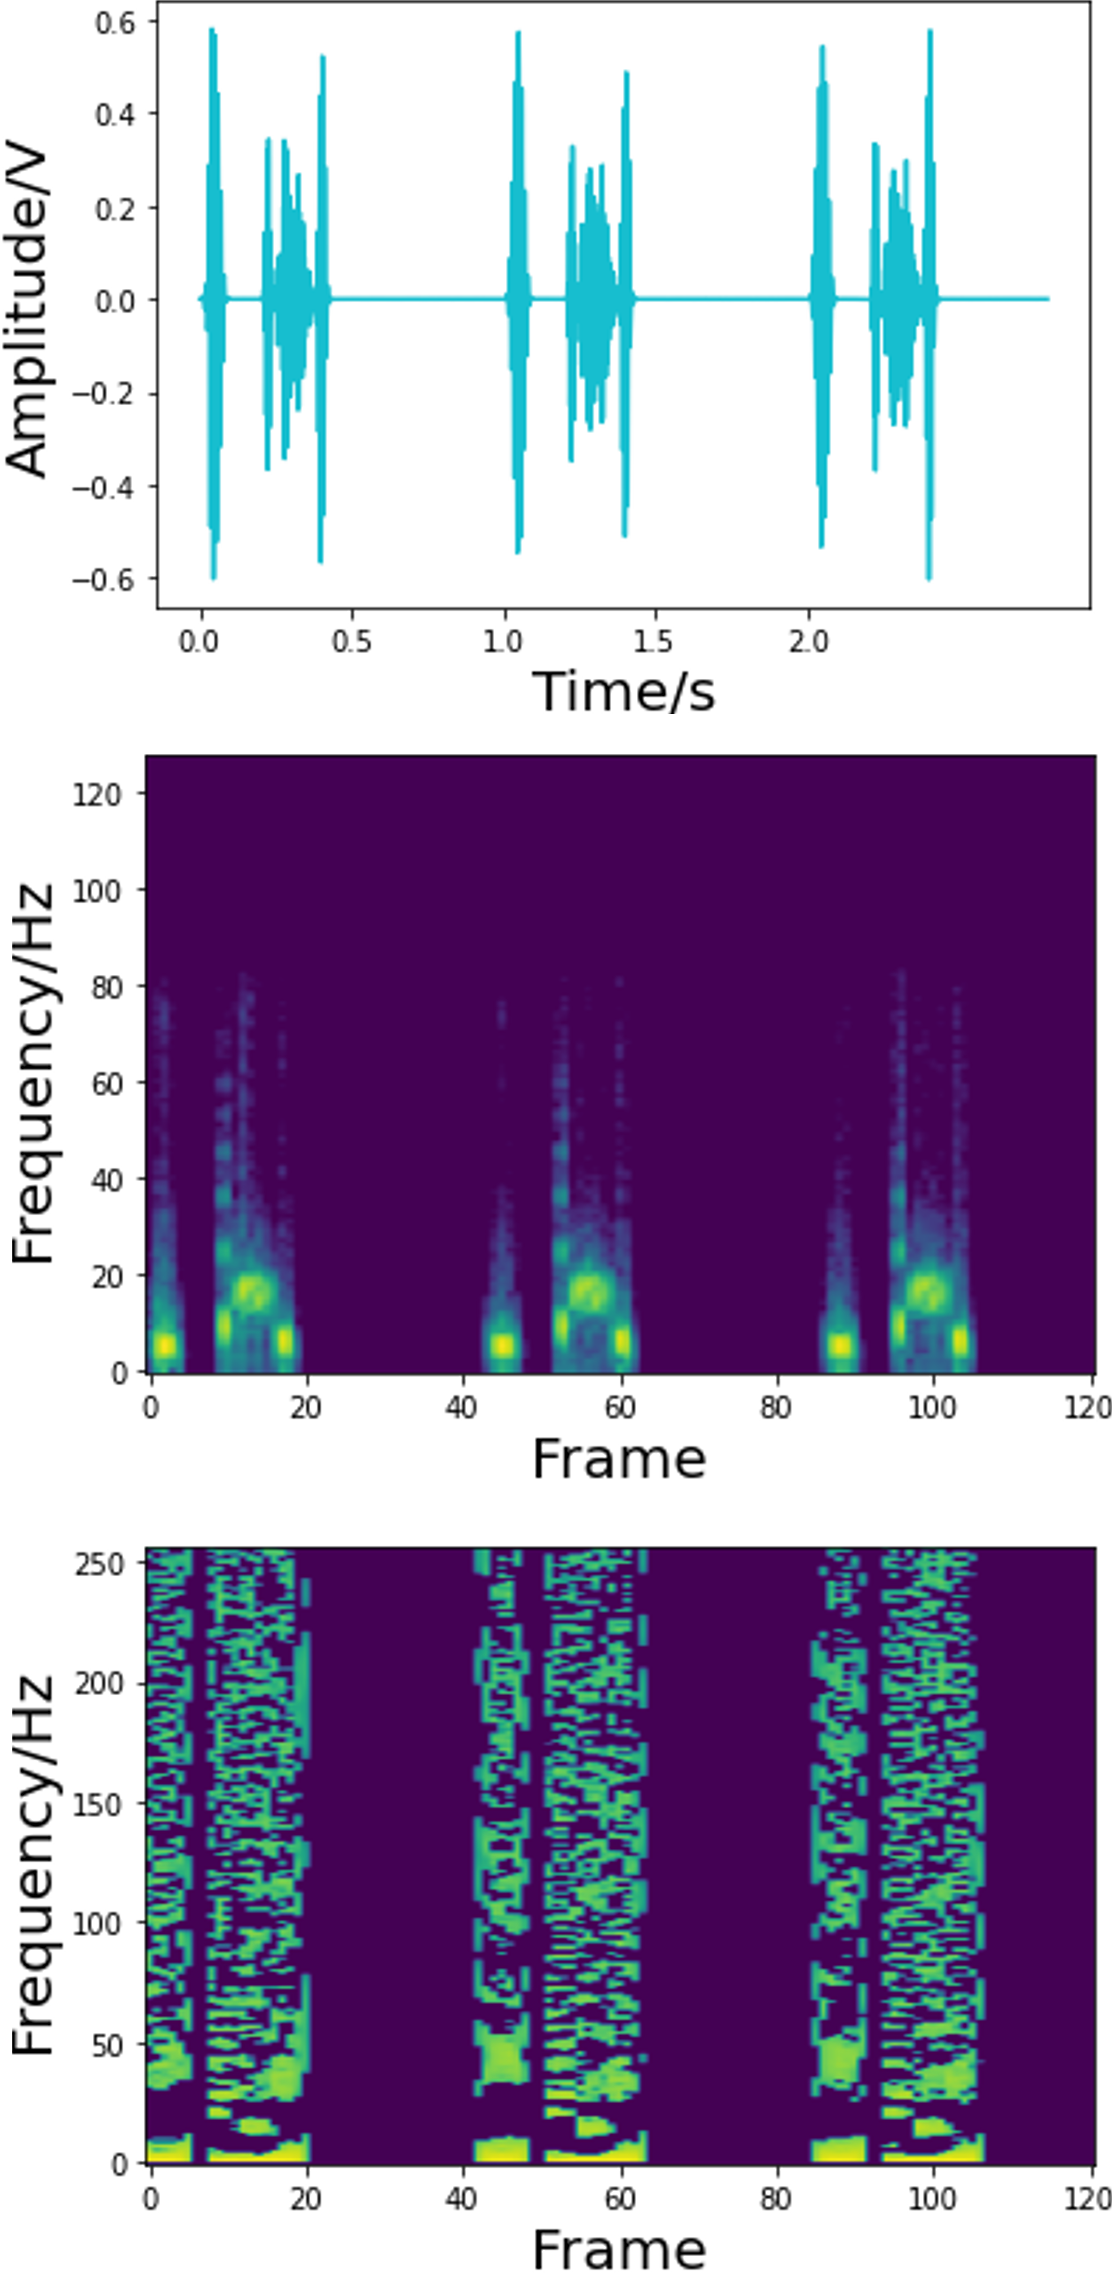
\includegraphics[width=1\linewidth]{figs/results/mvp_mfcc.png}
        \caption{Unhealthy heart sound}
        \label{FIG:mfcc.b}
    \end{subfigure}
\caption{\textbf{Feature extraction result}. (\textbf{a}) Waveform, Mel-spectrum, MFCC of normal heart sound. (\textbf{b}) Waveform, Mel-spectrum, MFCC of unhealthy MVP heart sound.}
\label{FIG:mfcc}
\end{figure}
% \subsubsection{Diagnostic performance}
% Tab. \ref{tab:HF Diagnosis 10-fold Results} presents the diagnostic outcomes for two heart failure diagnostic datasets and the publicly available Yaseen dataset.

% Previous researchers have also explored various intelligent algorithms for heart failure diagnosis or prediction, as shown in Tab. \ref{tab:Comparison}. Khade \cite{khade2019system} and Rao \cite{rao2022explainable} predicted heart failure incidence rates based on physiological parameters or medication records. Acharya \cite{acharya2019deep} and Matsumoto \cite{matsumoto2020diagnosing} examined the potential of diagnosing heart failure using ECG or X-ray images. In comparison to Khade \cite{khade2019system} and Rao \cite{rao2022explainable}, this paper offers enhanced medical diagnostic value and interpretability, along with Acharya \cite{acharya2019deep} and Matsumoto \cite{matsumoto2020diagnosing}. When compared to Acharya \cite{acharya2019deep} and Matsumoto \cite{matsumoto2020diagnosing}, this study theoretically boasts superior diagnostic speed, reduced device size, and more suitable application in ambulance settings.

% Compared with previous classification research efforts \cite{vepa2009classification, wu2010hidden, rubin2016classifying, arora2021transfer, li2021lightweight, shuvo2021cardioxnet}, this study incorporates several well-established and successful methods, including wavelet denoising, MFCC feature extraction, and the use of CNNs. We address the issue of signal processing and diagnosis in rapid short-duration auscultation. However, it lacks strong generalization capabilities in diagnosing mitral regurgitation, indicating that the model still suffers from overfitting problems. 
% Another limitation is the insufficient discussion of subtypes of AHF.

% \begin{table*}[h]
%  \caption{Comparison with other researches}
%   \label{tab:Comparison}
%     \centering
%     \begin{tabularx}{\textwidth}{ccccc}
%         \toprule
% 		 \multicolumn{5}{c}{\textbf{Comparison with other heart failure researches}}\\
%          \multicolumn{2}{c}{Authors} & \multicolumn{1}{c}{Dataset} & \multicolumn{1}{c}{Aim}& \multicolumn{1}{c}{Acc$(\%)$} \\
%         \midrule
%         \multicolumn{2}{c}{\textbf{Ours}} & \multicolumn{1}{c}{HF-Diagnosis dataset} & \multicolumn{1}{c}{HF diagnosis}& 99.25\\
%         \multicolumn{2}{c}{Khade \cite{khade2019system}} & \multicolumn{1}{c}{Physiological parameters}& \multicolumn{1}{c}{CHF prediction}& 88.30\\
%         \multicolumn{2}{c}{Rao \cite{rao2022explainable}} & \multicolumn{1}{c}{Medication records} & \multicolumn{1}{c}{CHF prediction}& 93.00\\
%         \multicolumn{2}{c}{Acharya \cite{acharya2019deep}} & \multicolumn{1}{c}{ECG} & \multicolumn{1}{c}{HF diagnosis}& 98.97\\
%         \multicolumn{2}{c}{Matsumoto \cite{matsumoto2020diagnosing}} & \multicolumn{1}{c}{X-Ray Images} & \multicolumn{1}{c}{HF diagnosis}  & 82.00\\
%         \toprule
% 		 \multicolumn{5}{c}{\textbf{Comparison with other heart sound researches}}\\
%         Authors & Feature extraction & Classification method & Databases & Acc$(\%)$ \\
%                 \midrule
%          \textbf{Ours} & MFCC & DenseHF-Net & Multi region fusion auscultation & 99.25 \\
%         \textbf{Ours} & MFCC & DenseHF-Net & Mitral valve auscultation & 92.60 \\
%         Chen \cite{chen2023robust} & STFT & CNN with Attention Mechanism & PhysioNet 2016& 94.12 \\
%         Xiang \cite{xiang2023research} & Logmel & Transfer Learning (MobileNet, Xception) &PhysioNet 2016& 90.23 \\
%         Vepa \cite{vepa2009classification} & STFT, DWT & kNN, MLP, SVM & Normal, systolic, diastolic records& 95.2\\
%         Vepa \cite{vepa2009classification} & STFT, DWT & kNN, MLP, SVM & Normal, systolic, diastolic records& 95.2\\
%         Wu \cite{wu2010hidden} & MFCC & HMM & 325 cycles of 10-type& 95.08 \\
%         Rubin \cite{rubin2016classifying} & MFCC & CNN & PhysioNet 2016& 95.2\\
%         Arora \cite{arora2021transfer} & STFT & CNN & PhysioNet 2016& 89.04\\
%         Li \cite{li2021lightweight} & STFT & CNN & PhysioNet 2016 & 85\\
%         Shuvo \cite{shuvo2021cardioxnet} & Time-invariant features &CNN & Yaseen database& 99.6\\
%         \bottomrule
%     \end{tabularx}
% \end{table*}
\subsubsection{Diagnostic performance}
Previous researchers have explored various intelligent algorithms for heart failure diagnosis or prediction, as shown in Tab. \ref{tab:Comparison}. For instance, Khade \cite{khade2019system} and Rao \cite{rao2022explainable} predicted heart failure incidence rates based on physiological parameters or medication records, while Acharya \cite{acharya2019deep} and Matsumoto \cite{matsumoto2020diagnosing} examined the potential of diagnosing heart failure using ECG or X-ray images. In comparison to these works, our study offers enhanced medical diagnostic value and interpretability, especially in ambulance settings, with superior diagnostic speed, reduced device size, and more suitable application.

Moreover, when compared to previous classification research efforts \cite{vepa2009classification, wu2010hidden, rubin2016classifying, arora2021transfer, li2021lightweight, shuvo2021cardioxnet}, this study incorporates well-established methods such as wavelet denoising, MFCC feature extraction, and CNNs, addressing issues of signal processing and diagnosis in rapid short-duration auscultation. However, challenges remain in the generalization capabilities for diagnosing mitral regurgitation, with the model still showing signs of overfitting. Additionally, the study lacks a thorough discussion of AHF subtypes.

In comparison, Chen \cite{chen2023robust} employed Short-Time Fourier Transform (STFT) as a feature extraction method combined with a CNN enhanced by an Attention Mechanism, achieving an accuracy of 94.12\% on the PhysioNet 2016 dataset. The introduction of the attention mechanism significantly improved the focus on relevant heart sound signal parts, leading to more accurate classifications. However, Chen's approach, while robust, increases computational costs, making it less suitable for real-time applications in resource-constrained environments like ambulances.

Xiang \cite{xiang2023research} explored Logmel features with Transfer Learning using pre-trained models such as MobileNet and Xception, achieving an accuracy of 90.23\% on the PhysioNet 2016 dataset. Though slightly underperforming in accuracy compared to Chen’s method, Xiang's approach offers better generalization and adaptability to different datasets with minimal additional training. The use of lightweight models like MobileNet is particularly promising for deployment in mobile and low-power devices, making it a suitable choice for real-time diagnostic applications.

In summary, while both Chen and Xiang have made significant contributions to heart sound classification, their methods cater to different needs: Chen's approach excels in accuracy through an attention-enhanced CNN, albeit with higher computational intensity, while Xiang's method offers a balance between performance and efficiency, particularly suitable for mobile and real-time applications.



\begin{table*}[h]
 \caption{Comparison with other researches}
  \label{tab:Comparison}
    \centering
    \begin{tabularx}{\textwidth}{ccccc}
        \toprule
        \multicolumn{5}{c}{\textbf{Comparison with other heart failure researches}}\\
        \multicolumn{2}{c}{Authors} & \multicolumn{1}{c}{Dataset} & \multicolumn{1}{c}{Aim} & \multicolumn{1}{c}{Acc$(\%)$} \\
        \midrule
        \multicolumn{2}{c}{\textbf{Ours}} & \multicolumn{1}{c}{HF-Diagnosis dataset} & \multicolumn{1}{c}{HF diagnosis} & 99.25 \\
        \multicolumn{2}{c}{Khade \cite{khade2019system}} & \multicolumn{1}{c}{Physiological parameters} & \multicolumn{1}{c}{CHF prediction} & 88.30 \\
        \multicolumn{2}{c}{Rao \cite{rao2022explainable}} & \multicolumn{1}{c}{Medication records} & \multicolumn{1}{c}{CHF prediction} & 93.00 \\
        \multicolumn{2}{c}{Acharya \cite{acharya2019deep}} & \multicolumn{1}{c}{ECG} & \multicolumn{1}{c}{HF diagnosis} & 98.97 \\
        \multicolumn{2}{c}{Matsumoto \cite{matsumoto2020diagnosing}} & \multicolumn{1}{c}{X-Ray Images} & \multicolumn{1}{c}{HF diagnosis} & 82.00 \\
        \midrule
        \multicolumn{5}{c}{\textbf{Comparison with other heart sound researches}}\\
        Authors & Feature extraction & Classification method & Databases & Acc$(\%)$ \\
        \midrule
        \textbf{Ours} & MFCC & DenseHF-Net & Multi region fusion auscultation & 99.25 \\
        \textbf{Ours} & MFCC & DenseHF-Net & Mitral valve auscultation & 92.60 \\
        Chen \cite{chen2023robust} & STFT & CNN with Attention Mechanism & PhysioNet 2016 & 94.12 \\
        Xiang \cite{xiang2023research} & Logmel & Transfer Learning (MobileNet, Xception) & PhysioNet 2016 & 90.23 \\
        Vepa \cite{vepa2009classification} & STFT, DWT & kNN, MLP, SVM & Normal, systolic, diastolic records & 95.20 \\
        Wu \cite{wu2010hidden} & MFCC & HMM & 325 cycles of 10-type & 95.08 \\
        Rubin \cite{rubin2016classifying} & MFCC & CNN & PhysioNet 2016 & 95.20 \\
        Arora \cite{arora2021transfer} & STFT & CNN & PhysioNet 2016 & 89.04 \\
        Li \cite{li2021lightweight} & STFT & CNN & PhysioNet 2016 & 85.00 \\
        Shuvo \cite{shuvo2021cardioxnet} & Time-invariant features & CNN & Yaseen database & 99.60 \\
        \bottomrule
    \end{tabularx}
\end{table*}
